\documentclass[11pt]{article}
\usepackage[T1]{fontenc}
\usepackage[utf8]{inputenc}
\usepackage{lmodern}
\usepackage[margin=1in]{geometry}
\usepackage{amsmath,amssymb,mathtools}
\usepackage{booktabs,longtable,array}
\usepackage{fancyvrb}
\usepackage[hidelinks]{hyperref}
\usepackage{microtype}
\usepackage{graphicx}
\usepackage{adjustbox}
\pdfinfoomitdate=1
\pdftrailerid{}
\pdfsuppressptexinfo=15
\setlength{\parindent}{0pt}
\setlength{\parskip}{0.6em}
\setlength{\emergencystretch}{3em}
\renewcommand{\arraystretch}{1.25}
\setlength{\tabcolsep}{4pt}
\sloppy
\graphicspath{{Revision/universe_model/}}
\title{UM-1 version 1.3: the gaps found by the analysis, and how they are closed}
\author{dirac16complex project (with Claude Opus 5.5)}
\date{}
\begin{document}
\maketitle
\tableofcontents
\newpage

Version 1 of 2026-10-17, written at the author's instruction of 2026-10-17: "Then go ahead, fix the gaps and push". The gaps are those found by the analysis \texttt{ANALYSIS.\allowbreak{}md} (its section 10) and those listed in \texttt{MODEL.\allowbreak{}md} section 8 and \texttt{SOLUTION.\allowbreak{}md} section 7. The computations are in \texttt{analysis/\allowbreak{}gap\_\allowbreak{}fixes.\allowbreak{}py} (4 of 4 checks PASS, \texttt{analysis/\allowbreak{}reports/\allowbreak{}gap-{}\allowbreak{}fixes-{}\allowbreak{}checks.\allowbreak{}json}), and the tables of section 7 are generated by it. The model changes are version 1.3 of \texttt{MODEL.\allowbreak{}md}; the origin of every new ingredient is in \texttt{PROVENANCE.\allowbreak{}md} section 8. The labels are those of \texttt{MODEL.\allowbreak{}md}: DERIVED, TAKEN, STANDARD, ASSUMED, INVENTED, OPEN, CHANGED; ESTIMATE and FROM MEMORY as in \texttt{ANALYSIS.\allowbreak{}md}. The coordinates are the author's, $X = \{x_0, x_1, \dots, x_7\}$, with $x_0$ the hidden space-like direction.

\section*{1. Summary: the gaps and their status}
\addcontentsline{toc}{section}{1. Summary: the gaps and their status}

\begin{longtable}{>{\raggedright\arraybackslash}p{0.198\linewidth}>{\raggedright\arraybackslash}p{0.137\linewidth}>{\raggedright\arraybackslash}p{0.198\linewidth}>{\raggedright\arraybackslash}p{0.320\linewidth}}
\toprule
\textbf{gap} & \textbf{found in} & \textbf{what version 1.3 does} & \textbf{status} \\
\midrule
the light masses ($W$, $Z$, $e$, $u$, $d$, $\nu$) did not come from the $x_0$ dependence of the wave functions but from tip terms & \texttt{ANALYSIS.\allowbreak{}md} 5, 6 & resolves the tip as a thin $x_0$ layer: the masses become the $x_0$ gradient energy of the wave functions, $m^2 = P_{tip}\langle\hat p^2\rangle_{tip}$; the fermion masses become exact $x_0$ eigenvalues (section 2) & CLOSED (DERIVED; the layer's inner structure is INVENTED and only its strength is physical) \\
the dark-matter reading and the $N_{eff}$ reading of the vector portal were in tension; the relic abundance was not derived & \texttt{ANALYSIS.\allowbreak{}md} 8.4, 8.5 & the vector portal P1 acts on the lepton multiplets only; the portal fixed by $N_{eff}$ then PREDICTS the dark-matter abundance (section 3) & CLOSED as a benchmark (INVENTED choice; ESTIMATE accuracy) \\
the docstring of \texttt{solution/\allowbreak{}masses.\allowbreak{}py} gave the wrong $f$ scaling of the tip parameter & \texttt{ANALYSIS.\allowbreak{}md} 3.3 & corrected (section 4) & CLOSED \\
the stability of the dark matter rests on the exact fold parity & \texttt{ANALYSIS.\allowbreak{}md} 8.3 & stated as a symmetry requirement of the full model & ASSUMED (unchanged) \\
dark energy: no $\Psi$ state qualifies & \texttt{ANALYSIS.\allowbreak{}md} 9 & none possible within the model: $\delta\Lambda$ stays & OPEN (the cosmological-constant problem) \\
no Higgs while a 125 GeV boson is observed; $WW$ unitarity near 1.2 TeV & \texttt{SOLUTION.\allowbreak{}md} 7 & inherent in the order ("do NOT include the Higgs particle") & CONFLICT (unchanged) \\
further open items & section 5 & listed & OPEN \\
\bottomrule
\end{longtable}

\section*{2. G1: every mass as the $x_0$ dependence of the wave function}
\addcontentsline{toc}{section}{2. G1: every mass as the $x_0$ dependence of the wave function}

\subsection*{2.1 The gauge bosons: the resolved tip (check G1a)}
\addcontentsline{toc}{subsection}{2.1 The gauge bosons: the resolved tip (check G1a)}

The analysis showed that $m_W^2$ is 99.87 \% a tip term of the sigma field: the Robin condition $u'(-1) = \beta u(-1)$ at the regular tip. A Robin condition is the thin-layer limit of a Dirichlet condition. Add beyond the tip a layer $t \in [-1-\delta, -1]$ of stiffness $w_\delta = \beta e^{-3\eta}\delta$, and let the broken-generator profiles vanish at its outer edge (symmetry breaking by a boundary condition, as in Higgsless models). A linear drop of $u$ across the layer has gradient energy $w_\delta u(-1)^2/\delta = \beta e^{-3\eta}u(-1)^2$, which is exactly the tip term. The mass of the $W$ is then

\[\adjustbox{max width=\linewidth}{$\displaystyle m_W^2 = \frac{\int dy\,w(y)\,|\partial_s u|^2}{\int dy\,w(y)\,|u|^2} = P_{tip}\,\langle\hat p^2\rangle_{tip} + (\text{bulk bending}),\qquad \langle\hat p^2\rangle_{tip} \geq \Big(\frac{\pi}{2\,\delta_s}\Big)^2 ,$}\]

where $P_{tip}$ is the probability of finding the $W$ in the layer and $\delta_s = fL\delta$ its proper thickness. The bound is the Poincaré inequality of a profile that must vanish within $\delta_s$: the precise form of the author's uncertainty argument.

The finite-element computation (1500 bulk and 300 layer elements; table of section 7.1) gives these results:
\begin{itemize}
\item the layered problem reproduces the Robin eigenvalue for $\delta = 10^{-2}, 10^{-3}, 10^{-4}$ to $3$ to $5\times10^{-5}$, the discretisation error;
\item the whole of $m_W^2$ is the $x_0$ gradient energy of the wave function, 99.868 \% of it inside the layer;
\item $P_{tip}$ falls like $\delta$ and $\langle\hat p^2\rangle_{tip}\delta^2 = 3.0$ stays above $(\pi/2)^2 = 2.47$;
\item the uncertainty bound alone gives $P_{tip}(\pi/2)^2/\delta^2 = 0.82\,m_W^2$.
\end{itemize}

The same holds for the $Z$.

So the $W$ is light although its wave function has a large hidden momentum where it varies. The variation is confined to the tip, where the probability of finding the $W$ is suppressed by the warp ($e^{-3\eta} = 1.2\times10^{-4}$ in the weight) and by the thinness of the layer. In this form the author's mechanism holds exactly: the mass is generated by the $x_0$ dependence of the wave function, and the uncertainty relation holds where that dependence sits, weighted by the probability of being there. The inner structure of the layer is INVENTED and is not resolved by UM-1; every layer with the same $w_\delta/\delta$ gives the same masses.

\begin{figure}[htbp]
\centering
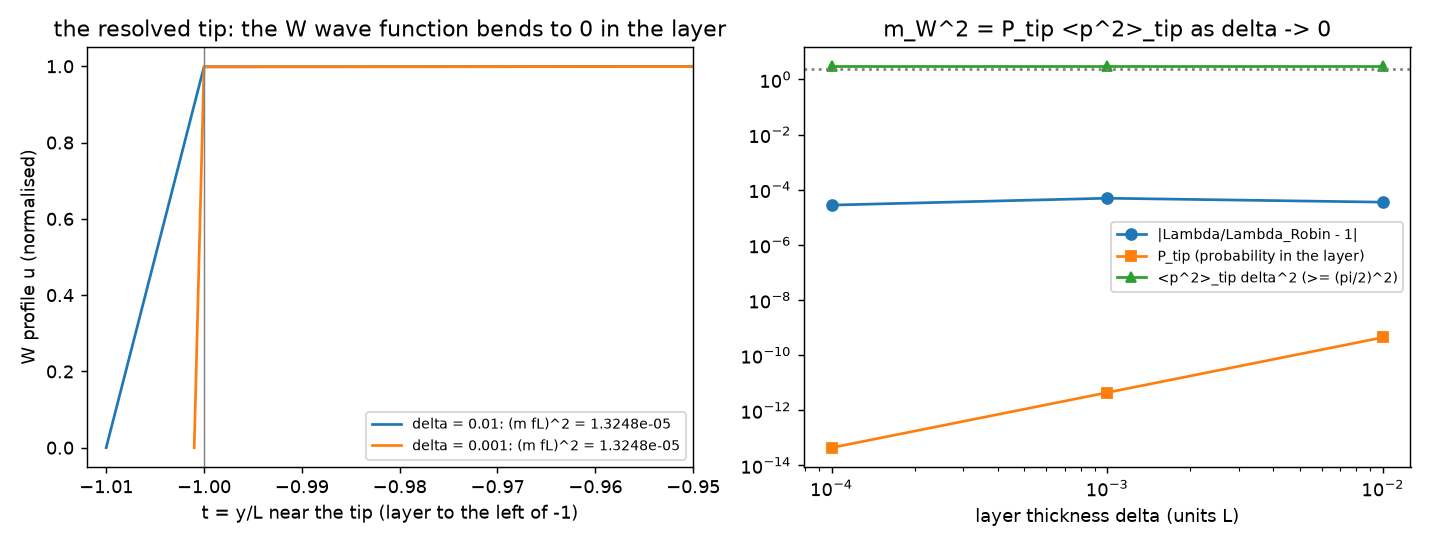
\includegraphics[width=0.85\linewidth]{analysis/figures/figC1_resolved_tip.png}
\caption{The resolved tip: the W profile bends to zero inside the tip layer; the eigenvalue, the layer probability and the layer momentum as the layer thins.}
\end{figure}

\subsection*{2.2 The fermions: exact $x_0$ eigenvalues (check G1b)}
\addcontentsline{toc}{subsection}{2.2 The fermions: exact $x_0$ eigenvalues (check G1b)}

The tip Yukawa coupling of \texttt{MODEL.\allowbreak{}md} section 4.3 mixes the left-handed and right-handed zero modes at the tip. As a condition on the coupled $(L, R)$ $x_0$ Dirac problem it reads

\[b_L(-1) = \kappa\, b_R(-1),\qquad a_R(-1) = -\kappa\, a_L(-1) .\]

This is the self-adjoint mixing condition; its boundary form $\sum_{L,R}\varphi^\dagger\sigma_1\psi$ vanishes. The fold conditions are unchanged ($b_L(0) = 0$, $a_R(0) = 0$). The four-dimensional mass is the lowest eigenvalue of this $x_0$ problem. It is computed exactly with closed-form transfer matrices (mpmath, 50 digits; table of section 7.2). With $\kappa = \sqrt{\Lambda_1} = 5.488$ (the $\lambda_f = 1$ of \texttt{SOLUTION.\allowbreak{}md}):
\begin{itemize}
\item the exact eigenvalue equals the first-order value $\kappa\,\zeta(c_L)\zeta(c_R)$ to $5.8\times10^{-8}$ (the $d$ quark; the correction is $O(\kappa^2e^{-2c})$);
\item it reproduces the observed $e$, $u$, $d$, $\nu$ masses to $10^{-6}$;
\item for a broad mode ($c = 1$) the exact eigenvalue lies 24.7 \% below first order.
\end{itemize}

The fermion masses of UM-1 are therefore exact $x_0$ eigenvalues of their wave functions. The mass is the tip mixing times the amplitudes of the two chiral wave functions at the tip, $\zeta(c)^2$, the probability density there.

\subsection*{2.3 The precise form of the author's principle (DERIVED, version 1.3)}
\addcontentsline{toc}{subsection}{2.3 The precise form of the author's principle (DERIVED, version 1.3)}

For every field of UM-1, the four-dimensional mass is the $x_0$ dependence of its wave function measured relative to the geometric zero mode:

\[\adjustbox{max width=\linewidth}{$\displaystyle m^2 = \sum_{\text{regions}} P_{\text{region}}\,\langle\hat p^2\rangle_{\text{region}}\quad(\text{dressed hidden momentum}),\qquad \langle\hat p^2\rangle_{\text{region}} \geq \frac{\hbar^2}{4\,\Delta s^2}\ \text{or}\ \Big(\frac{\pi\hbar}{2\,\delta_s}\Big)^2 .$}\]

\begin{itemize}
\item MASSLESS: the profile is flat relative to the geometry ($u = $ const, or $h\chi = 0$): the graviton, the photon, the gluons and the fold-band quanta of $\Psi$. The author's exception list, extended by the gluons.
\item HEAVY: the $x_0$ dependence fills the cell, $P \approx 1$, so $m \geq 3H/(2f) = 99.4$ TeV. These are the Kaluza-Klein modes, the odd modes and the $\Psi$ bulk band; the dark matter (50.9 TeV) is the lightest odd state.
\item LIGHT: the $x_0$ dependence sits at the tip, $P_{tip} \ll 1$. These are $W$, $Z$, $e$, $u$, $d$ and $\nu$.
\end{itemize}

\section*{3. G2: the dark-matter abundance from the $N_{eff}$ portal (check G2)}
\addcontentsline{toc}{section}{3. G2: the dark-matter abundance from the $N_{eff}$ portal (check G2)}

\subsection*{3.1 The change}
\addcontentsline{toc}{subsection}{3.1 The change}

\texttt{MODEL.\allowbreak{}md} version 1.3 (CHANGED, INVENTED choice): the vector portal P1 acts on the lepton multiplets only, $\frac{c_V}{\Lambda_D^6}(\bar\Psi\gamma^M\Psi)(\bar\psi\gamma_M\psi)$ with $\psi \in \{L, e_R\}$. Each multiplet's operator is separately gauge invariant, so this is consistent with the electroweak theory. $\Psi$ keeps its interactions with the quarks through the other portals:
\begin{itemize}
\item P2: the scalar tip portal, suppressed by $\zeta_q^2$;
\item P5: the covariant-derivative contact, proportional to $m_q$ on shell;
\item P3: the dipole, through the photon and the $Z$;
\item P4: the $Z$ portal.
\end{itemize}

The order's "new CRITICAL interactions" with photons, neutrinos, electrons, quarks, $W$ and $Z$ are all still present.

\subsection*{3.2 The prediction}
\addcontentsline{toc}{subsection}{3.2 The prediction}

The fold band decouples in the QCD crossover for $N_{eff} = 2.99$ (\texttt{SOLUTION.\allowbreak{}md} section 6). Its vector portal is $G^{-1/2} = 12.3$ TeV (neutrino-like estimate; the targets of the decoupling are the leptons, as for neutrinos). The dark matter couples to the same portal with its $x_0$ overlap, 0.329 of the fold band's (\texttt{ANALYSIS.\allowbreak{}md} section 8.5), so $G^{-1/2} = 21.5$ TeV. It annihilates into $e$ (Dirac) and $\nu_L$ (chiral), 1.5 Dirac-equivalent channels, with $\sigma v = G^2M^2/\pi$ per channel (\texttt{ANALYSIS.\allowbreak{}md} check B2). The result is

\[\adjustbox{max width=\linewidth}{$\displaystyle \langle\sigma v\rangle = 1.04 \times \langle\sigma v\rangle_{relic},\qquad \Omega_{DM}h^2 = 0.115\,\Big(\frac{T_{dec}}{150\ \text{MeV}}\Big)^3 ,$}\]

i.e. $0.059$ to $0.199$ for $T_{dec} = 120$ to $180$ MeV. Planck's $0.120$ is reached at $T_{dec} = 152$ MeV. The dark-matter abundance is no longer a free input: it follows from the requirement $N_{eff} = 2.99$, the dark-matter mass of 50.9 TeV and the $x_0$ profiles. The agreement holds within the accuracy of the decoupling estimate (a factor of about 2 from $T_{dec}$ alone) (ESTIMATE).

\begin{figure}[htbp]
\centering
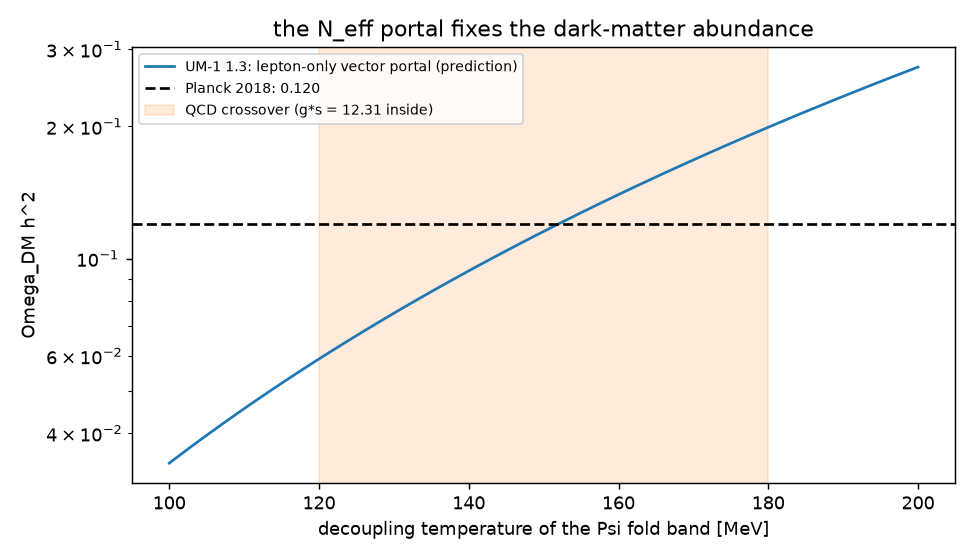
\includegraphics[width=0.85\linewidth]{analysis/figures/figC2_relic_prediction.png}
\caption{The dark-matter abundance predicted by the N\_eff portal against the decoupling temperature of the fold band; Planck's value lies inside the QCD crossover.}
\end{figure}

\subsection*{3.3 Detection and the remaining requirements}
\addcontentsline{toc}{subsection}{3.3 Detection and the remaining requirements}

\begin{itemize}
\item Direct detection only through the electron loop, i.e. photon mixing (ESTIMATE, the formula of Kopp et al. 2009, FROM MEMORY). The result is $\sigma_{SI} = 7.7\times10^{-50}$ cm$^2$ per xenon nucleon, $3\times10^{-5}$ of the LZ limit. The tension of \texttt{ANALYSIS.\allowbreak{}md} section 8.5 is gone.
\item CMB energy injection (into $e^+e^-$): $p_{ann} = 5.3\times10^{-31}$ cm$^3$/s/GeV against the bound $3.2\times10^{-28}$ (Planck 2018, FROM MEMORY).
\item REQUIRED: the annihilation into fold-band pairs through $\lambda$, which is p-wave for the scalar-scalar part, stays below $6.7\times10^{-26}$ cm$^3$/s; otherwise the dark matter is under-abundant. The quark couplings of P2 and P5 must respect the direct-detection limit; P2 is suppressed by $\zeta_q^2 \sim 10^{-8}$.
\item Unchanged: the fold-band decoupling, hence $N_{eff}$, the CNB and the BAO fit of \texttt{SOLUTION.\allowbreak{}md} section 6. The dark matter decouples kinetically from the leptons long before recombination, so at the CMB it behaves as cold dark matter, and the fitting-formula treatment stands.
\end{itemize}

\section*{4. G3: the tip parameter in \texttt{solution/\allowbreak{}masses.\allowbreak{}py} (check G3)}
\addcontentsline{toc}{section}{4. G3: the tip parameter in \texttt{solution/\allowbreak{}masses.\allowbreak{}py} (check G3)}

The docstring now states $\beta = c\,\hat g^2v_\Sigma^2fL$, proportional to $f$, as derived in \texttt{ANALYSIS.\allowbreak{}md} section 3.3. The fitted $\beta$ and every number of the solution are unchanged.

\section*{5. What remains open}
\addcontentsline{toc}{section}{5. What remains open}

\begin{itemize}
\item The fold parity must be exact, to $2\times10^{-27}$ in amplitude (ASSUMED).
\item The reduction of $\lambda(\bar\Psi\Psi)^2$ to four-dimensional couplings and the size of the $\lambda$ channel (OPEN).
\item Dark energy is $\delta\Lambda/H^2 = 7.5\times10^{-93}$, tuned. No state of $\Psi$ can supply it (OPEN; the cosmological-constant problem).
\item No Higgs boson; $WW$ unitarity near 1.2 TeV, below $m_{KK}$ (CONFLICT, inherent in the order).
\item The block stabiliser (the Casimir energy of the cell) and the transition from the primordial deflation to the static block, which must end before nucleosynthesis (OPEN).
\item The CMB at the level of a Boltzmann code; the $S$ parameter of the Higgsless tip; the anomalies of the eight-dimensional bulk theory; the second and third generations (OPEN).
\end{itemize}

\section*{6. Changes to the other documents}
\addcontentsline{toc}{section}{6. Changes to the other documents}

\begin{itemize}
\item \texttt{MODEL.\allowbreak{}md} version 1.3:
\begin{itemize}
\item section 4.4: the resolved tip and the precise principle;
\item section 4.5: P1 on the lepton multiplets;
\item section 8: CHANGED (1.3);
\item section 9: the summary.
\end{itemize}
\item \texttt{SOLUTION.\allowbreak{}md} version 1.2: sections 4.2 (fermion masses as exact eigenvalues), 6 (the predicted abundance) and 7.
\item \texttt{ANALYSIS.\allowbreak{}md} section 10: a pointer to this document.
\item \texttt{PROVENANCE.\allowbreak{}md} version 1.3: section 8, the provenance of the gap fixes.
\item \texttt{README.\allowbreak{}md}; the gate step um1-analysis-gaps; um1-pdfs builds this document.
\end{itemize}

\section*{7. Results}
\addcontentsline{toc}{section}{7. Results}

\subsection*{7.1 The resolved tip (\texttt{analysis/\allowbreak{}outputs/\allowbreak{}gap\_\allowbreak{}fixes.\allowbreak{}json})}
\addcontentsline{toc}{subsection}{7.1 The resolved tip (\texttt{analysis/\allowbreak{}outputs/\allowbreak{}gap\_\allowbreak{}fixes.\allowbreak{}json})}

\begingroup\small
\begin{longtable}{>{\raggedright\arraybackslash}p{0.076\linewidth}>{\raggedright\arraybackslash}p{0.123\linewidth}>{\raggedright\arraybackslash}p{0.146\linewidth}>{\raggedright\arraybackslash}p{0.127\linewidth}>{\raggedright\arraybackslash}p{0.123\linewidth}>{\raggedright\arraybackslash}p{0.114\linewidth}>{\raggedright\arraybackslash}p{0.114\linewidth}}
\toprule
\textbf{boson} & \textbf{$\delta$} & \textbf{$(mfL)^2$} & \textbf{deviation from the Robin value} & \textbf{$P_{tip}$} & \textbf{$\langle p^2\rangle_{tip}\delta^2$} & \textbf{layer share of the gradient energy} \\
\midrule
$W$ & 0.01 & $1.32476\times10^{-5}$ & $3.5\times10^{-5}$ & $4.41\times10^{-10}$ & 3 & 0.998678 \\
$W$ & 0.001 & $1.32478\times10^{-5}$ & $4.9\times10^{-5}$ & $4.41\times10^{-12}$ & 3 & 0.998678 \\
$W$ & $1.000\times10^{-4}$ & $1.32475\times10^{-5}$ & $2.8\times10^{-5}$ & $4.41\times10^{-14}$ & 3 & 0.998678 \\
$Z$ & 0.01 & $1.70476\times10^{-5}$ & $2.4\times10^{-5}$ & $5.67\times10^{-10}$ & 3 & 0.998298 \\
$Z$ & 0.001 & $1.70477\times10^{-5}$ & $2.8\times10^{-5}$ & $5.67\times10^{-12}$ & 3 & 0.998298 \\
$Z$ & $1.000\times10^{-4}$ & $1.70477\times10^{-5}$ & $2.8\times10^{-5}$ & $5.67\times10^{-14}$ & 3 & 0.998298 \\
\bottomrule
\end{longtable}
\endgroup

\subsection*{7.2 The fermion masses as exact $x_0$ eigenvalues}
\addcontentsline{toc}{subsection}{7.2 The fermion masses as exact $x_0$ eigenvalues}

\begin{longtable}{>{\raggedright\arraybackslash}p{0.110\linewidth}>{\raggedright\arraybackslash}p{0.073\linewidth}>{\raggedright\arraybackslash}p{0.171\linewidth}>{\raggedright\arraybackslash}p{0.171\linewidth}>{\raggedright\arraybackslash}p{0.152\linewidth}>{\raggedright\arraybackslash}p{0.171\linewidth}}
\toprule
\textbf{fermion} & \textbf{$c_f$} & \textbf{exact $\varepsilon fL$} & \textbf{$\kappa\zeta^2$} & \textbf{relative difference} & \textbf{$m$ [GeV]} \\
\midrule
$e$ & 11.2 & $2.31415\times10^{-8}$ & $2.31415\times10^{-8}$ & $-5.7\times10^{-9}$ & $5.10999\times10^{-4}$ \\
$u$ & 10.44 & $9.78194\times10^{-8}$ & $9.78194\times10^{-8}$ & $-2.6\times10^{-8}$ & 0.00216 \\
$d$ & 10.03 & $2.12848\times10^{-7}$ & $2.12848\times10^{-7}$ & $-5.8\times10^{-8}$ & 0.0047 \\
$\nu$ & 19.54 & $2.26434\times10^{-15}$ & $2.26434\times10^{-15}$ & $-3.3\times10^{-16}$ & $5.00000\times10^{-11}$ \\
\bottomrule
\end{longtable}

\subsection*{7.3 The lepton-only vector portal}
\addcontentsline{toc}{subsection}{7.3 The lepton-only vector portal}

\begin{longtable}{>{\raggedright\arraybackslash}p{0.465\linewidth}>{\raggedright\arraybackslash}p{0.421\linewidth}}
\toprule
\textbf{quantity} & \textbf{value} \\
\midrule
fold-band portal for $N_{eff} = 2.99$, $G^{-1/2}$ & 12.3 TeV \\
dark-matter portal (overlap 0.329), $G^{-1/2}$ & 21.5 TeV \\
$\langle\sigma v\rangle$ into $e$, $\nu$ / relic value & 1.04 \\
predicted $\Omega_{DM}h^2$ at $T_{dec} = 150$ MeV & 0.115 \\
$\Omega_{DM}h^2$ at $T_{dec}$ = 120 MeV & 0.059 \\
$\Omega_{DM}h^2$ at $T_{dec}$ = 135 MeV & 0.084 \\
$\Omega_{DM}h^2$ at $T_{dec}$ = 150 MeV & 0.115 \\
$\Omega_{DM}h^2$ at $T_{dec}$ = 165 MeV & 0.153 \\
$\Omega_{DM}h^2$ at $T_{dec}$ = 180 MeV & 0.199 \\
$T_{dec}$ for $\Omega h^2 = 0.120$ & 152 MeV \\
$\sigma_{SI}$ per xenon nucleon (electron loop) & $7.7\times10^{-50}$ cm$^2$ ($2.8\times10^{-5}$ of the limit) \\
CMB energy injection $p_{ann}$ & $5.3\times10^{-31}$ cm$^3$/s/GeV (bound $3.2\times10^{-28}$) \\
\bottomrule
\end{longtable}


\section*{8. Reproduction}
\addcontentsline{toc}{section}{8. Reproduction}

From the repository root, after the analysis (\texttt{ANALYSIS.\allowbreak{}md} section 11), under \texttt{timeout -{}\allowbreak{}k 5 423}:

\begin{Verbatim}[fontsize=\small]
cd Revision/universe_model
python analysis/gap_fixes.py          # about 15 s, 4 checks; section 7
python tools/build_pdfs.py GAPS
\end{Verbatim}

\end{document}
